\documentclass{article}
\usepackage[utf8]{inputenc} %кодировка
\usepackage[T2A]{fontenc}
\usepackage[english,russian]{babel} %русификатор 
\usepackage{mathtools} %библиотека матеши
\usepackage[left=1cm,right=1cm,top=2cm,bottom=2cm,bindingoffset=0cm]{geometry} %изменение отступов на листе
\usepackage{amsmath}
\usepackage{graphicx} %библиотека для графики и картинок
\graphicspath{}
\DeclareGraphicsExtensions{.pdf,.png,.jpg}
\usepackage{subcaption}
\usepackage{pgfplots}
\usepackage{amssymb}
\usepackage{physics}

\begin{document}
% НАЧАЛО ТИТУЛЬНОГО ЛИСТА
\begin{center}
    \Large
    Федеральное государственное автономное \\
    образовательное учреждение высшего образования \\ 
    «Научно-образовательная корпорация ИТМО»\\
    \vspace{0.5cm}
    \large
    Факультет программной инженерии и компьютерной техники \\
    Направление подготовки 09.03.04 Программная инженерия \\
    \vspace{1cm}
    \Large
    \textbf{Отчёт по лабораторной работе №3} \\
    По дисциплине «Базы данных» (второй семестр)\\
    \large
    \vspace{8cm}

    \begin{minipage}{.33\textwidth}
    \end{minipage}
    \hfill
    \begin{minipage}{.4\textwidth}
    
        \textbf{Студент}: \vspace{.1cm} \\
        \ Дениченко Александр P3112\\
        \textbf{Практик}:  \\
        \ Лисицина В.В
    \end{minipage}
    \vfill
Санкт-Петербург\\ 2023 г.
\end{center}

% КОНЕЦ ТИТУЛЬНОГО ЛИСТА 
\newpage

\section{Векторная ФНП и векторное поле}
\begin{equation*}
    \overline{\mathcal{V}} = (\mathcal{V}_x; \mathcal{V}_y) = (\mathcal{V}_x(x;y);\mathcal{V}_y(x,y)) = \mathcal{V}_x(x;y)\overline{i}+\mathcal{V}_y(x,y)\overline{j}
\end{equation*}
$\Psi$ \textbf{Вектор-функцией в области D называется вектор, координатами которого являются функции, заданные в этой области}
\begin{equation*}
    \overline{F}(x;y) = (P(x;y); Q(x;y)) = P(x;y)\overline{i}+Q(x;y)\overline{j}\ \ in \ \mathbb{R}^2
\end{equation*}
\begin{equation*}
    \overline{F}(x;y;z) = (P(x;y); Q(x;y); R(x;y)) = P(x;y)\overline{i}+Q(x;y)\overline{j}+R(x;y)\overline{k}\ \ in \ \mathbb{R}^2
\end{equation*}
Векторное поле в $\mathcal{D}$
\\
График - поле направлений
\\
Линия в каждой точке, которой векторное поле касается неё, называется векторной линией этого поля.

\textbf{Example}
\begin{equation*}
    \overline{F}(x;y) = (x+y;x-y);\ P(x;y) = x+y;\ Q(x;y) = x-y
\end{equation*}
Найдём векторные линии
\begin{equation*}
    y=y(x);\ tg\alpha = y' = \frac{Q}{P}
\end{equation*}
\begin{equation*}
    y'= \frac{x-y}{x+y};\ \ y^2+2xy-x^2=C;\ \ C\in\mathbb{R}
\end{equation*}

\section{Градиент скалярного поля}
\begin{equation*}
    z(x;y)\ diff\ in \mathcal{D}^2
\end{equation*}
\begin{equation*}
    M \in \mathcal{D}:\ (\pdv{z}{x}\ (M); \pdv{z}{y}\ (M)) = \pdv{z}{x}\overline{i}+\pdv{z}{y}\overline{j} = grad\ z\ (M)
\end{equation*}
\begin{equation*}
    u(x;y;z)\ diff\ in \mathcal{D}^3
\end{equation*}
\begin{equation*}
    M \in \mathcal{D}:\ (\pdv{u}{x}; \pdv{u}{y}; \pdv{u}{z}) = grad\ u\ (M)
\end{equation*}
\textbf{Example}
\begin{equation*}
    z= \frac{1}{2}(x^2+y^2);\ grad\ z=(x;y)
\end{equation*}
\begin{equation*}
    \overline{g}_1 = grad\ z(1;0) = (1; 0)
\end{equation*}
\begin{equation*}
    \overline{g}_2 = grad\ z(0;1) = (0; 1)
\end{equation*}
\begin{equation*}
    \overline{g}_3 = grad\ z(3;1) = (3; 1)
\end{equation*}
\begin{center}
    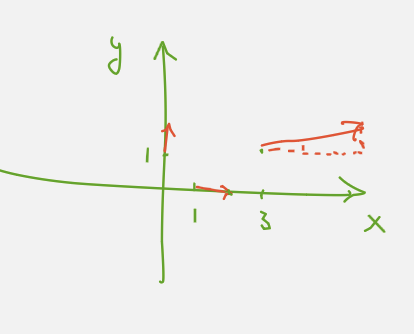
\includegraphics[width=.3\textwidth]{grad.png} 
\end{center}
Векторные линии:
\begin{equation*}
    y' = \frac{y}{x}\ \ \dv{y}{x}= \frac{y}{x}\ \ \frac{dy}{y}= \frac{dx}{x}\ \ \int\frac{dy}{y} = \int\frac{dx}{x}
\end{equation*}
\begin{equation*}
    ln|y| = ln|x| + C;\ C = ln|C_1|
\end{equation*}
\begin{equation*}
    |y|= |C_1x|
\end{equation*}
\begin{equation*}
    y= C_1x,\ C_1\in \mathbb{R}
\end{equation*}
\begin{center}
    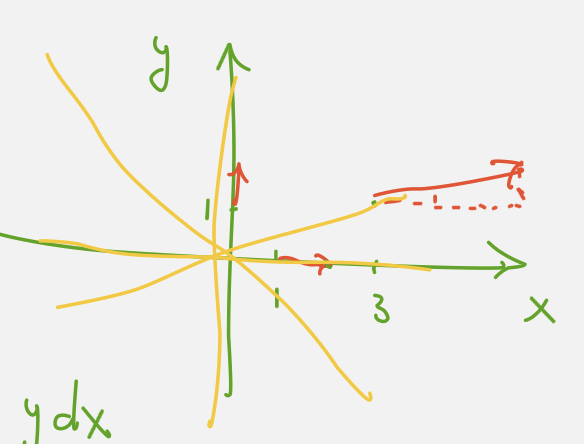
\includegraphics[width=.3\textwidth]{ans_grad.png} 
\end{center}
Свойства градиента:\\
1) Градиент скалярной функции z(x;y) каждой точке направлен перпендикулярно к линии уровня z(x;y), проходящей через эту точку.

Доказательство:

\begin{equation*}
    z = z(x;y)\ \ z(x;y) = C - level\ line
\end{equation*}
\begin{equation*}
    k_1 = y' = -\frac{z'_x}{z'_y} - \text{угловой коэфицент касательной к линии уровня}
\end{equation*}
\begin{equation*}
    grad\ z(x;y) = (z'_x; z'_y)
\end{equation*}
\begin{equation*}
    k_2 = \frac{z'_y}{z'_x}
\end{equation*}
\begin{equation*}
    k_1\cdot k_2 = -\frac{z'_x}{z'_y}\cdot \frac{z'_y}{z'_x} = -1
\end{equation*}

2)Линейность
\begin{equation*}
    grad(f+g) = grad(f)+ grad(g)
\end{equation*}
\begin{equation*}
    grad(\alpha f)  =\alpha grad(f), \alpha\cdot\in \mathbb{R}
\end{equation*}
3)
\begin{equation*}
    grad(f\cdot g) = f\cdot grad(g) + g\cdot grad(f)
\end{equation*}
4)
\begin{equation*}
    \pdv{z}{l}= \text{проекция grad(z)}
\end{equation*}
Докажем
\begin{equation*}
    \pdv{z}{l}= \pdv{z}{x}cos\alpha+\pdv{z}{y}cos\beta = (\pdv{z}{x}; \pdv{z}{y})\cdot (cos\alpha;cos\beta) = gradz\cdot \overline{l}^o = |grad\ z|\cdot |\overline{l}^o|\cdot cos\phi = |grad\ z|\cdot \phi 
\end{equation*}
\begin{equation*}
    \phi = \angle (grad\ z; \overline{l}^o)
\end{equation*}
По какой траектории движется точка P при изменении направления $\overline{l}$?
\begin{center}
    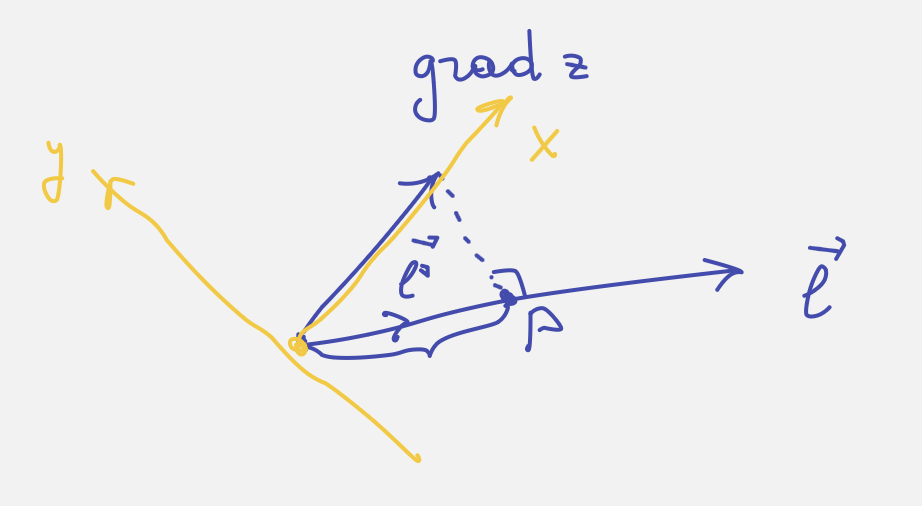
\includegraphics[width=.3\textwidth]{gradx.png}
\end{center}
P = (x;y) - точка
\begin{equation*}
    x = \pdv{z}{l}\cdot \cos\phi
\end{equation*}
\begin{equation*}
    y = \pdv{z}{l}\cdot \sin\phi
\end{equation*}
\begin{equation*}
    \pdv{z}{l} = |grad\ z|\cdot \cos\phi
\end{equation*}
\begin{equation*}
\begin{cases}

        x = |grad\ z|\cdot \cos^2\phi\\

        y = |grad\ z|\cdot \cos\phi \sin\phi

\end{cases}->\ 
\begin{cases}

    x = \frac{1}{2}|grad\ z|\cdot (1+cos2\phi)\\

    y = |grad\ z|\cdot \sin2\phi

\end{cases}->\ 
\begin{cases}

    (x-\frac{|g|}{2})^2 = (\frac{1}{2}|g|\cdot cos2\phi)^2\\

    y^2 = (\frac{1}{2}|grad\ z|\cdot \sin2\phi)^2

\end{cases}
\end{equation*}

\begin{equation*}
    \left(x - \frac{|g|}{2}\right)^2+y^2 = \frac{|g|^2}{4}
\end{equation*}
окружность с центром в $(\frac{|g|}{2};0)\ and R = \frac{|g|}{2}$ 

доказано
5) 
\begin{equation*}
    \pdv{z}{l}, \ \overline{l} = grad(z),\ = maximum
\end{equation*}
6)
\begin{equation*}
    \pdv{z}{l}, \ \overline{l} \bot  grad(z),\  = 0
\end{equation*}
\textbf{Example}

Найти наибольшую крутизну(угол наклона поверхности) подъёма поверхности

\begin{equation*}
    z = ln(x^2+2y^2) \ \ in\ \  M(6;4\sqrt{2};ln(100))
\end{equation*}
\begin{equation*}
    \pdv{z}{l} = |grad\ z| = tg\ \alpha
\end{equation*}
\begin{equation*}
    |grad\ z| = (\frac{2x}{x^2+2y^2}; \frac{4y}{x^2+2y^2})
\end{equation*}
\begin{equation*}
    grad\ z(M) = (\frac{12}{100};\frac{16\sqrt{2}}{100})
\end{equation*}
\begin{equation*}
    |grad\ z(M)| \approx  \frac{1}{4} = tg\alpha
\end{equation*}
% 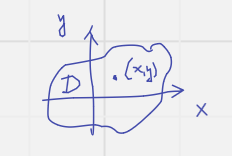
\includegraphics[width=.3\textwidth]{1.1} 
\end{document}
